% chapter09.tex

 %%%%%%%%%%%%%%%%%%%%%%%%%%%%%%%%%%%%%%%%%%%%%%%%%%%%%%%%%%%%%%%%%%%%%%%%%%%%%
 %                                                                           %
 %    PyMS documentation                                                     %
 %    Copyright (C) 2005-2010 Vladimir Likic                                 %
 %                                                                           %
 %    The files in this directory provided under the Creative Commons        %
 %    Attribution-NonCommercial-NoDerivs 2.1 Australia license               %
 %    http://creativecommons.org/licenses/by-nc-nd/2.1/au/                   %
 %    See the file license.txt                                               %
 %                                                                           %
 %%%%%%%%%%%%%%%%%%%%%%%%%%%%%%%%%%%%%%%%%%%%%%%%%%%%%%%%%%%%%%%%%%%%%%%%%%%%%

\chapter{Parallel processing with PyMS}

\section{\label{sec:mpi}Requirements}

Using PyMS parallel capabilities requires installation of the package
'mpi4py', which provides bindings of the Message Passing Interface (MPI)
for the Python programming language. This package can be downloaded
from {\tt http://code.google.com/p/mpi4py/}. Since 'mpi4py' provides
only Python bindings, it requires an MPI implementation. We recommend
using mpich2:\\
{\tt http://www.mcs.anl.gov/research/projects/mpich2/}\\
We show the installation of 'mpich2' and 'mpi2py' on Linux system from
software distributions downloaded from the projects' web site.

\subsection{\label{sec:mpich2}Installation of 'mpich2'}

\begin{enumerate}

\item From the mpich2 project web site download the current distribution of
mpich2 (in our case the file 'mpich2-1.2.1p1.tar.gz').

\item Prepare the directory for mpich2 installation. In this example
we have chosen to use /usr/local/mpich2/. Our version of mpitch2 is
1.2.1, and to allow for the installation of different version later,
we create a subdirectory "1.2.1",

\begin{verbatim}
$ mkdir -vp /usr/local/mpich2/1.2.1
\end{verbatim}

The above command will make the directory /usr/local/mpich2/ and also
/usr/local/mpich2/1.2.1. Note that /usr/local is usually owned by
root, and the above commands may require root privileges.

\item Unpack this file and change to the source code directory:

\begin{verbatim}
$ tar xvfz mpich2-1.2.1p1.tar.gz 
$ cd  mpich2-1.2.1p1
\end{verbatim}

\item Configure, compile, and install mpich2:

\begin{verbatim}
$ ./configure --prefix=/usr/local/mpich2/1.2.1 --enable-sharedlibs=gcc
$ make
$ make install
\end{verbatim}

If /usr/local/mpich2/1.2.1 is owned by rood, the above command
may require root privileges.

\end{enumerate}

\subsection{\label{sec:mpi4py}Installation of 'mpi4py'}

\begin{enumerate}

\item From the mpi4py project web site download the current distribution
of mpi4py (in our case the file 'mpi4py-1.2.1.tar.gz').

\item Unpack this file and change to the source code directory:

\begin{verbatim}
$ tar xvfz mpi4py-1.2.1.tar.gz
$ cd mpi4py-1.2.1
\end{verbatim}

\item Edit the file 'mpi.cfg' to reflect the location of mpich2.  In
our case this file after editing contained the following:

\begin{verbatim}
# MPICH2
[mpi]
mpi_dir              = /usr/local/mpich2/1.2.1
mpicc                = %(mpi_dir)s/bin/mpicc
mpicxx               = %(mpi_dir)s/bin/mpicxx
\end{verbatim}

\item Install mpi4py:

\begin{verbatim}
$ python setup.py install
\end{verbatim}

\item Check that mpi4py works:

\begin{verbatim}
$ python
Python 2.5.2 (r252:60911, Sep 10 2008, 14:39:22) 
[GCC 4.1.1 20070105 (Red Hat 4.1.1-52)] on linux2
Type "help", "copyright", "credits" or "license" for more information.
>>> import mpi4py
>>> 
\end{verbatim}

If the above command import produced no output, mpi4py is installed
properly and ready to use.

\end{enumerate}

\section{\label{sec:parallel-background}Background to using PyMS in parallel}

Any processing that loops through ion chromatograms or mass spectra can
be performed in parallel, by distributing the processing of individual
ion chromatograms or mass spectra to different CPUs by using the
efficient MPI mechanism.

Before the parallel processing can be deployed, data needs to be binned
to produce an IntensityMatrix object, as described in the Section
\ref{sec:intensity-matrix}. This is essentially a two dimensional
matrix, with ion chromatograms along one dimension and mass spectra
along the other dimension.

Consider the processing which applies a noise smoothing function to
each ion chromatogram. We first read the raw data:

\begin{verbatim}
andi_file = "/x/PyMS/data/gc01_0812_066.cdf"
data = ANDI_reader(andi_file)
\end{verbatim}
 
Then build the intensity matrix, and get its dimensions:

\begin{verbatim}
im = build_intensity_matrix_i(data)
n_scan, n_mz = im.get_size()
\end{verbatim}

The last command sets the variables n\_scan and n\_mz to the number
scans and number of m/z values present in data, respectively.
Processing of ion chromatograms with the noise smoothing function
requires fetching of each ion chromatogram from the data, and
application of the noise smoothing function. This can be achieved 
with a simple loop: 

\begin{verbatim}
for ii in n_mz:
    print ii+1,
    ic = im.get_ic_at_index(ii)
    ic_smooth = window_smooth(ic, window=7)
\end{verbatim}

This example epitomizes the typical processing required on the
GC-MS data. Another, equally important processing, is that of
individual mass spectra. In this case the same logic can be
applied, except that one would loop over the other dimension
of the IntensityMatrix object 'im'. That is, one would loop
over all the scan indices, and use the method 
get\_ms\_at\_index() to fetch individual mass spectra:


\begin{verbatim}
for ii in n_scan:
    print ii+1,
    ms = im.get_ms_at_index(ii)
    # here do something the the mass spectra 'ms'
\end{verbatim}

Processing of data in this fashion is computationally intensive.
A typical data set may consist of 3,000-10,000 scans and ~500
m/z values. If complex processing algorithms are applied to
each ion chromatogram (or mass spectra), the processing will
quickly become computationally prohibitive.

The type of calculation illustrated above is an ideal candidate
for parallelization because each ion chromatogram (or mass
spectrum) are processed independently. PyMS takes advantage
of this and allows one to harvest the power of multiple CPUs
to speed-up the processing. To achieve this PyMS can distributes
the loop from the above (either type, ie. over ion chromatograms
or mass spectra) over the available CPUs, achieving a linear
speed-up with the number of CPUs.


\section{\label{sec:parallel-pyms}Using PyMS in parallel}

Using PyMS in parallel requires a minimal intervention, only
that special method of the IntensityMatrix object is invoked
in the for loop described above. For looping over all ion
chromatograms in parallel,

\begin{verbatim}
for ii in im.iter_ic_indices():
    print ii+1,
    ic = im.get_ic_at_index(ii)
    ic_smooth = window_smooth(ic, window=7)
\end{verbatim}

The only change is that 

\begin{verbatim}
for ii in n_mz:
\end{verbatim}

is replaced with

\begin{verbatim}
for ii in im.iter_ic_indices()
\end{verbatim}

The corresponding method for looping over all mass spectra
would involve replacing:

\begin{verbatim}
for ii in n_scan:
\end{verbatim}

with

\begin{verbatim}
for ii in im.iter_ms_indices()
\end{verbatim}

The special constructs {\tt for ii in im.iter\_ic\_indices():} and
{\tt for ii in im.iter\_ms\_indices()} will distribute the calculation
in parallel if MPI capability is available (ie. mpi4py is installed
on the system, and multiple CPUs are available). If MPI capability
is not available, the processing will be performed in a serial mode.
Running in parallel also requires some prior preparations, as explained
below.

Consider how the following script that performs noise smoothing example
described above (named 'proc.py'). This script is can be run in serial
or parallel mode.

\begin{verbatim}
"""proc.py
"""

import sys
sys.path.append("/x/PyMS")

from pyms.GCMS.IO.ANDI.Function import ANDI_reader
from pyms.GCMS.Function import build_intensity_matrix_i
from pyms.Noise.Window import window_smooth

# read the raw data as a GCMS_data object
andi_file = "/x/PyMS/data/gc01_0812_066.cdf"
data = ANDI_reader(andi_file)

# build the intensity matrix
im = build_intensity_matrix_i(data)

# get the size of the intensity matrix
n_scan, n_mz = im.get_size()
print "Size of the intensity matrix is (n_scans, n_mz):", n_scan, n_mz

# loop over all m/z values, fetch the corresponding IC, and perform
# noise smoothing
for ii in im.iter_ic_indices():
    print ii+1,
    ic = im.get_ic_at_index(ii)
    ic_smooth = window_smooth(ic, window=7)
\end{verbatim}

A simple running of this script will produce a serial run without
any warning messages:

\begin{verbatim}
$ python proc.py
 -> Reading netCDF file '/x/PyMS/data/gc01_0812_066.cdf'
Size of the intensity matrix is (n_scans, n_mz): 9865 551
1 2 3 4 5 6 7 8 9 10 11 12 13 14 15 16 17 18 19 20 21 22 23 24 25
26 27 28 29 30 31 32 33 34 35 36 37 38 39 40 41 42 43 44 45 46 47
... [ further output deleted ] ...
\end{verbatim}

Inspection of the CPU usage during the execution of the program
shows that only one CPU is utilised 100\% (although multiple CPUs
are available) as shown in Figure \ref{fig:top-serial}.

\begin{figure}
  \begin{center}
    
\includegraphics[scale=1.0]{graphics/chapter09/top-serial.eps}
  \end{center}
  \caption{The xterm output of the program 'top' with PyMS running in
  serial mode on the computer with multiple CPUs}
  \label{fig:top-serial}
\end{figure}

To run the above script in parallel, one needs first to start the
mpitch2 process launcher, called 'mpd' (this is a program, in this
example located in\\
 {\tt /usr/local/mpich2/1.2.1/bin/mpd},\\
see the section \label{sec:mpitch2}). This can be achieved as follows:

\begin{verbatim}
$ /usr/local/mpich2/1.2.1/bin/mpd --daemon
\end{verbatim}

The above command start 'mpd' as a daemon (the program runs in the
background, without a controlling terminal).  A common problem
that causes the above command is fail is the absence of the
{\tt .mpd.conf
\begin{figure}
  \begin{center}
    
\includegraphics[scale=1.0]{graphics/chapter09/top-serial.eps}
  \end{center}
  \caption{The xterm output of the program 'top' with PyMS running in
  serial mode on the computer with multiple CPUs}
  \label{fig:top-serial}
\end{figure}
} file which 'mpd' requires to be present in the
home directory of the user who is starting the process. Here is
an excerpt from the 'mpd' help page:

\begin{verbatim}
A file named .mpd.conf file must be present in the user's home directory
with read and write access only for the user, and must contain at least
a line with MPD_SECRETWORD=<secretword>
To run mpd as root, install it while root and instead of a .mpd.conf file
use mpd.conf (no leading dot) in the /etc directory.' 
\end{verbatim}

Fixing this problem is simple, and requires creating the file
{\tt ~/.mpd.conf}, which in our case contains only one line:

\begin{verbatim}
MPD_SECRETWORD=euSe0veo
\end{verbatim}

After this the 'mpd' can be launched.  Running the PyMS script in the parallel
mode requires the use of 'mpirun' command,

\begin{verbatim}
$ /usr/local/mpich2/1.2.1/bin/mpirun -np 2 python proc.py 
\end{verbatim}

The above command prepare 'python proc.py' to run in parallel, in this
case by using two CPUS ({\tt -np 2}). The execution produces the
following output:

\begin{verbatim}
$ /usr/local/mpich2/1.2.1/bin/mpirun -np 2 python proc.py 
 -> Reading netCDF file '/x/PyMS/data/gc01_0812_066.cdf'
 -> Reading netCDF file '/x/PyMS/data/gc01_0812_066.cdf'
Size of the intensity matrix is (n_scans, n_mz):Size of
the intensity matrix is (n_scans, n_mz): 9865 551
276 9865 551
1 277 2 278 3 279 4 280 5 281 6 282 7 283 8 284 9 285 10 286 11 287 12
288 13 289 14 290 15 291 16 292 17 293 18 294 19 295 20 296 21 297 22
298 23 299 24 300 25 301 26 302 27 303 28 304 2
... [ further output deleted ] ...
\end{verbatim}

The above shows that two processes are active (each reading its own
version of data). While the distribution of processing between the
two processes has been achieved automatically by PyMS. Since both
processes were started from the same terminal their output is
intermingled. This time the processing is using two CPUs, and this
can be seen from the inspection of CPU utilisation, as shown in
Figure \ref{fig:top-parallel}. Also the execution of the script
'proc.py' is now two times faster.

\begin{figure}
  \begin{center}
    
\includegraphics[scale=1.0]{graphics/chapter09/top-parallel.eps}
  \end{center}
  \caption{The xterm output of the program 'top' with PyMS running in
  parallel mode with two CPUs}
  \label{fig:top-parallel}
\end{figure}

This simple example shows how to speed-up PyMS processing on a common
workstation with two CPUs. The MPI also allows PyMS processing to run
on specialised computers with many CPUs, such as Linux clusters. The
MPI implementation allows PyMS to be easily used in such distributed
computing environments, much like in the example above. We have tested
PyMS on Linux clusters, and the resulting speed-up is nearly linear
with the number of CPUs employed (Figure \ref{fig:speedup-parallel}).

\begin{figure}
  \begin{center}
    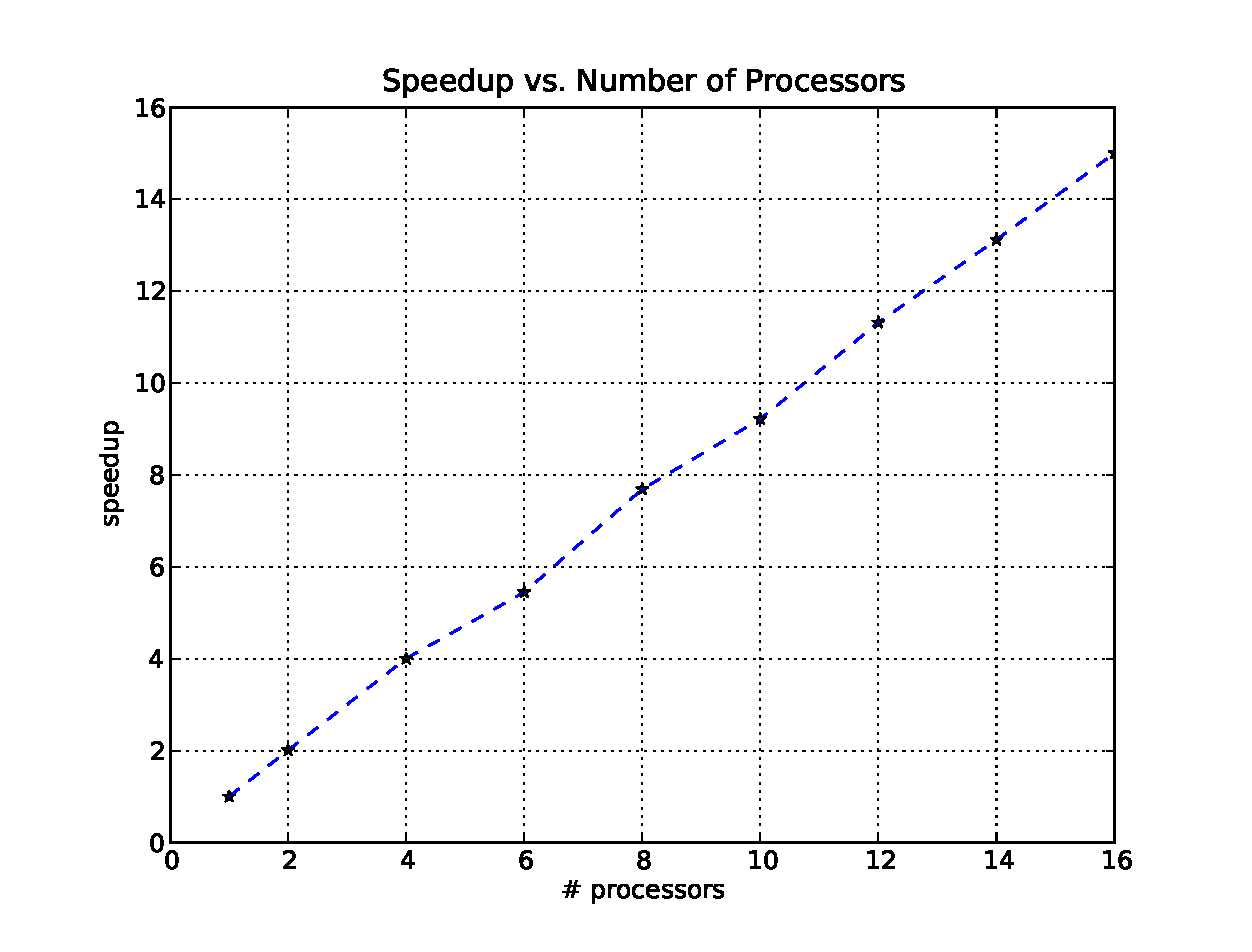
\includegraphics[scale=0.5]{graphics/chapter09/speedup-parallel.eps}
  \end{center}
  \caption{The speedup in PyMS processing when run in parallel on a Linux
  cluster as a function of a number of CPUs deployed}
  \label{fig:speedup-parallel}
\end{figure}

